\chapter{Electromagnetic Worldlines: Numerical Forces and Curvatures
for the TE Polarization}
\label{ch:force}

The preceding work has focused on computing the Casimir energy between dielectric bodies.  However,
a number of experiments directly measure the force, or even the second spatial derivative of the energy.
Experiments that detect the shift in frequency of an oscillator, such as 
measuring the motion of a BEC in a harmonic trap~\citep{Harber2005,Obrecht2007}, or  
a nanoelectromechanical oscillators~\citep{Chan2001}, are sensitive the curvature of the Casimir energy.

As already noted in Section~\ref{sec:finite_difference}, the finite difference method has some drawbacks
when applied to worldline path integrals.  
Derivatives of discontinuous functions such as those required in worldline path integrals lead to large statistical errors.
In Section~\ref{sec:partial_averaging}, we developed specialized techniques for handling derivatives of Casimir--Polder 
energies.  This chapter develops a parallel discussion for computing the force on macroscopic bodies.  

Prior investigations by \citet{Weber2009, Weber2010} computed the Casimir force in the worldline method for
the Dirichlet boundary conditions.
They computed the force between a planar surface and a cylindrical or spherical body, and the
torque between inclined plates.  Their methods typically rely on finding analytical expressions for 
the path times $\cT$ when a particular Brownian path will intersect the surfaces, and analytically integrate over 
the path time $\cT$ and path starting position $\vect{x}_0$.  

In contrast, our approach to the worldline method has also emphasized Monte Carlo integration over
the path time and starting position.  
In Section~\ref{sec:path-pinning}, we derive the ``pinning'' approach, where the forces emerge from
paths that are pinned to start on the surfaces of the relevant bodies.  
This approach is used to derive worldline expressions for the force~(\ref{eq:pinning_force}),
 potential curvature~(\ref{eq:potential_curvature}) and torque~(\ref{eq:pinning_torque}).
%In these expressions the forces emerge from paths that are just touch the bodies, or are ``pinned'' to the surfaces.
Unfortunately, when $\chi/N\gg 1$ the pinning expressions give too small an answer, which prompts developing the 
``occupation'' method in Section~\ref{sec:occupation}.  
Using the occupation method, we can derive alternative expressions for the force~(\ref{eq:occupation_force}), 
potential curvature~(\ref{eq:curvature_occupy}) and torque~(\ref{eq:torque_occupy}).  These expressions
also make contact with the approach used by \citet{Weber2009,Weber2010}.
These occupation expressions still work at large $\chi/N$,
but some care is needed to sample from all of the relevant classes of paths at both weak~($\chi/N\ll 1$) 
and strong~($\chi/N\gg 1$) coupling.
Section~\ref{sec:force_numerics} discusses the numerical simulations for planar media where the correspondence
to the TE polarization can be exploited.
We find that even the occupation methods of Section~\ref{sec:occupation} can fail at strong coupling.  
However, this is due to the strong-coupling limit requiring a rare set of paths which just ``graze'' the
bodies.
This can be confronted by either using a large ensemble of paths, or adjusting
the sampling procedure to explicitly capture the strong-coupling limit.  
In Section~\ref{sec:generic_coupling}, a ``general-$\chi$'' approach is used
for small $\chi$, and in Section~\ref{sec:softened_delta} one possible approach to capturing the strong-coupling
limit is presented.  

The results in this chapter are explicitly derived for
the TE worldline path integral, although presumably these results can be generalized to the TM worldline path integral.
That could be done by exploiting the partial averaging methods discussed in Section~\ref{sec:partial_averaging}.
The partial averaging is necessary since directly evaluating the derivatives on the path-averaged 
TM potential~(\ref{eq:TM_pot}) leads to terms like $(d-x_k)/\Delta \cT$.
Those terms have large statistical fluctuations as $\Delta \cT\rightarrow 0$, but partial averaging 
could mitigate those fluctuations.  
[The results presented here, along with the material on partial averaging in Section~\ref{sec:partial_averaging}
is in preparation for publication.]

\section{Surface Pinned Paths}
\label{sec:path-pinning}

The renormalized TE Casimir energy was given in Eq.~(\ref{eq:TE_Casimir}). 
Although the energy was derived under the assumptions of describing electromagnetism in planar media,
it can be studied in its own right as a scalar field theory in arbitrary geometries of bodies. 
%It also serves as an uncontrolled approximation to the electromagnetic Casimir energy in general geometries.  
We will consider the following worldline path integral
\begin{equation}
  E = \frac{\hbar c}{2(2\pi)^{D/2}}\int_0^\infty \frac{d\cT}{\cT^{1+D/2}}
  \, W,
  \label{eq:spatial_path_integralE}
\end{equation}
% Since we will be computing derivatives of the Casimir energy with respect to distance, and angle,
% we can confine our attention to just the spatial part of the integral, which is schematically given 
% by
where the integrals over the spatial coordinates in the worldline path integral are given by
\begin{align}
  W &:= \int d\vect{x}_0
  \,\biggdlangle \frac{1}{\langle\epsr\rangle^a}-\frac{1}{[\epsr(\vect{x}_0)]^a}\biggdrangle_{\vect{x}(t)},
  \label{eq:spatial_path_integral}
\end{align}
where $a=1/2$ when applied to TE Casimir energies in planar geometries.    

In the following treatment 
we will consider a general geometry for computing Casimir forces between material bodies (Figure~\ref{fig:spud_sketch}).
For simplicity, we will assume uniform dielectric bodies
separated by vacuum.  % , to focus on the most problematic features
% of sharp, dielectric interfaces.  However, the treatment here
% may be straightforwardly generalized to nonuniform dielectric media.
In this case, the relative dielectric permittivity $\epsr(\vect{r})$ is given  by 
\begin{equation}
  \epsr(\vect{r}) = 1+\sum_j\chi_j\Theta[\sigma_j(\vect{r}-\vect{R}_j)],
\end{equation}
where $\chi_j$ is the dielectric susceptibility of body $j$;
$\sigma_j(\vect{r})=0$ 
defines the surface of the $j$th body, with $\sigma_j>0$ and $\sigma_j<0$ 
on the interior and exterior of the body,
respectively; and $\vect{R}_j$ is the center of the $j$th body.  
\begin{figure}
  \centering
  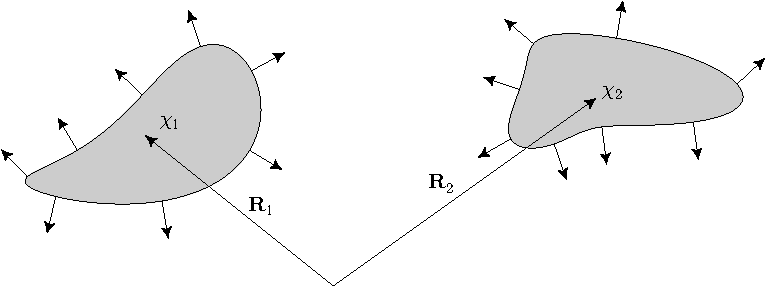
\includegraphics[width=0.6\columnwidth]{fig/spud_sketch}
  \caption[Sketch of geometry for interacting bodies]{
    Sketch of the geometry for interacting dielectric bodies of susceptibility $\chi_j$, centered at
    $\vect{R}_j$ relative to the origin.  The surface of the $j$th body is
    defined by the condition $\sigma_j=0$.
    The unit normal vectors $\hat{n}_j$ to the surface of the $j$th  body
    are also shown.}
  \label{fig:spud_sketch}
\end{figure}

\subsection{Force}
The force on a body follows from a gradient of the Casimir energy,
where the derivatives are taken with respect to the body's 
position.
For example, the components of the force on body $2$, expressed
with Cartesian basis vectors $\hat{r}_i$, are
given by directional derivatives of the path integral in Eqs.~(\ref{eq:spatial_path_integralE}) and 
(\ref{eq:spatial_path_integral}) with respect to
the components of the body position $\mathbf{R}_2$.  The resulting force is
\begin{align}
  &F_{2,i}:=-\frac{\hbar c}{2(2\pi)^{D/2}}\int_0^\infty \!\!\frac{d\cT}{\cT^{1+D/2}}\hat{r}_i\cdot\nablaR2 W
  \nonumber\\
   &\hspace{0.cm}=
   -\frac{a\chi_2\hbar c}{2(2\pi)^{D/2}}
   \!\!
   \int_0^\infty \!\!\!\frac{d\cT}{\cT^{1+D/2}}   \!\int \!d\vect{x}_0\, 
  \Biggdlangle \frac{
  \hat{r}_i\cdot\big\langle 
  \delta(\sigma_2)\,\nabla\sigma_2\big\rangle}
  {\langle\epsr\rangle^{a+1}}\Biggdrangle_{\!\vect{x}(t)}\!\!\!\!,
  \label{eq:forcepathint}
\end{align}
where $\sigma_2 = \sigma_2[\vect{x}(t)-\vect{R}_2]$ in this expression, and $\nablaR{i}$ denotes the gradient with
respect $\vect{R}_i$.
The path-averaged delta function acts to pin the paths to the surface where $\sigma_2=0$.
% The path integration can be simplified by viewing the delta function,
% whose argument involves $\vect{x}(t)$, as a constraint on the
% source point $\vect{x}_0$ of the paths.
Writing out the relevant part of the path integral (\ref{eq:forcepathint}),
the delta function reduces the $D$-dimensional integration
over $\vect{x}_0$ to a $(D-1)$-dimensional integration over
the surface of body 2, with the result
\begin{align}
  &\int d\vect{x}_0  \Biggdlangle \frac{
  \big\langle 
  \delta\big(\sigma_2[\vect{x}(t)-\vect{R}_2]\big)\,\nabla\sigma_2[\vect{x}(t)-\vect{R}_2]\big\rangle}
  {\langle\epsr\rangle^{a+1}}\Biggdrangle_{\vect{x}(t)} \nonumber\\
  % &\hspace{0.5cm}= 
  % \int d\vect{x}_0  \Biggdlangle \frac{
  % \delta\big(\sigma_2[\vect{x}_0-\vect{R}_2]\big)\,\nabla\sigma_2[\x0-\vect{R}_2]}
  % {\langle\epsr\rangle^{a+1}}\Biggdrangle_{\vect{x}(t)} \nonumber\\
  &\hspace{0.5cm}= 
  \oint\limits_{\sigma_2(\vect{x}_0-\vect{R}_2)=0}^{}
   \hspace{-3ex}
dS\hspace{1.5ex}\biggdlangle 
  \frac{\nabla\sigma_2(\x0-\vect{R}_2)}
  {\langle\epsr\rangle^{a+1}|\nabla\sigma_2(\x0-\vect{R}_2)|}\biggdrangle_{\vect{x}(t)},
  \label{eq:delta-normal}
\end{align}
where the final integral (over path source points $\vect{x}_0$)
is a surface integral over the 
surface of body 2.  % The first equality here can be understood
% in terms of a discrete path (i.e., in a ``time-slicing'' regularization
% of the path integral), where the path average in the numerator
% amounts to a sum of terms, each involving a delta function
% involving a path coordinate $\vect{x}_j$.  In the average over all
% paths and sum over all source points $\vect{x}_0$,
% the delta function is equivalently a function of the
% source point, since $\vect{x}_j$ is the source point
% of another equivalent path.
This relation follows from simplifying the path-averaged delta function using Eq.~(\ref{eq:delta_pin}),
and the result~\citep{Hormander1983} 
\begin{equation}
  \int d\mathbf{x}\, \delta[h(\vect{x})]\,f(\vect{x})
  = \int_{h^{-1}(0)} \!\!\!\!\!dS\,\frac{1}{|\nabla h(\vect{x})|}f(\vect{x}),
  \label{hormander1}
\end{equation}
where $S$ is the surface defined by $h(\vect{x})=0$, and 
\begin{equation}
|\nabla h(\vect{x})|=\Bigg[\sum_k \left(\frac{\partial h}{\partial x_k}\right)^2\Bigg]^{1/2}.
  \label{hormander2}
\end{equation}
% The 
% follows from an application of the H\"ormander formula
% (see Eq.~(22) in Ref.~\cite{Mackrory2016}).
The renormalized force vector can be found by summing over all force components, and subtracting 
the corresponding single-body force,
\begin{align}
  \vect{F}_{2}&=
  -\frac{a\chi_2\hbar c}{2(2\pi)^{D/2}}
\int\limits_0^\infty \!\frac{d\cT}{\cT^{1+D/2}}    
\hspace{-3ex}
 \oint\limits_{\sigma_2(\vect{x}_0-\vect{R}_2)=0}^{}
  \hspace{-4ex} dS\hspace{1ex} 
  \hat{n}_2(\vect{x}_0) % \nonumber\\
  % &\hspace{0.5cm}\times 
  \Biggdlangle\frac{1}{\langle\epsilon_{\mathrm{r},12}\rangle^{a+1}}-\frac{1}{\langle\epsilon_{\mathrm{r},2}\rangle^{a+1}}
  \Biggdrangle_{\vect{x}(t)},
  \label{eq:pinning_force}
\end{align}
where the unit-normal vector for the surface of body 2 is defined as
\begin{equation}
  \hat{n}_2(\x0) := -\frac{\nabla \sigma_2(\x0-\vect{R}_2)}{|\nabla \sigma_2(\x0-\vect{R}_2)|}.
\end{equation}
Qualitatively, the Casimir force on a body arises from 
paths that start on a body's surface.  The direction of the 
force from a small patch of the surface is determined by the local
surface normal. 
Since each patch is at different distances from the other bodies, 
the paths from each patch contribute at different path times.  Once the integral 
over the surface is carried out, this results in a net force on the body.  

\subsection{Potential Curvature}

This method can be easily extended to the second derivative of the worldline energy, which 
computes the potential curvature,  
\begin{equation}
  C_{ij} := (\hat{r}_i\cdot \nablaR2)(\hat{r}_j\cdot \nablaR2)E.
\end{equation}
For a dielectric describing two bodies, the gradients with respect to $\vect{R}_2$ can be rewritten 
in terms of gradients with respect to the first body's center $\vect{R}_1$, and the path coordinates $\vect{x}_k$,
\begin{align}
  \nablaR2\langle \epsr\rangle  
  =& \bigg(\sum_{k=1}^N\nablaxk-\nablaR1\bigg)% \nonumber\\
  % & \times
[\langle \epsilon_1(\vect{x}-\vect{R}_1)\rangle+\langle\epsilon_2(\vect{x}-\vect{R}_2)\rangle],
% \frac{\partial}{\partial R_{2,i}}\langle \epsr\rangle  
%   =& \bigg(\sum_{k=1}^N\frac{\partial}{\partial {x}_{k,i}}-\frac{\partial}{\partial R_{1,i}}\bigg)\nonumber\\
%   & \times[\langle \epsilon_1(\vect{x}-\vect{R}_1)\rangle+\langle\epsilon_2(\vect{x}-\vect{R}_2)\rangle],
  \label{eq:shift_derivative}
\end{align}
where $\nablaxk$ is the gradient of the path position $\vect{x}_k$.    
The first derivative can be carried out as before:
\begin{align}
  C_{ij} = &
\frac{a\chi_1\hbar c}{2(2\pi)^{D/2}}\intzinf \frac{d\cT}{\cT^{1+D/2}}
\int d\vect{x}_0 
\biggdlangle 
\hat{r}_{i}\!\cdot\!\bigg(\!\sum_k\nablaxk - \nablaR{1}\!\bigg)
  \!
  \frac{\big[\hat{r}_{j}\cdot\langle \nabla\sigma_2\delta(\sigma_2)\rangle\big]}
  {\langle\epsr\rangle^{a+1}}\biggdrangle_{\vect{x}(t)}.
\end{align}
% \begin{align}
%   C_{ij} = &
% \frac{-a(a+1)\chi_2\hbar c}{2(2\pi)^{D/2}}\intzinf \frac{d\cT}{\cT^{1+D/2}}
% \int d\vect{x}_0 % \nonumber\\
% % &\hspace{0.05cm}\times
% \biggdlangle 
% \big(\hat{r}_{i}\cdot\langle \delta(\sigma_1)\nablaR{1}\sigma_1\rangle\big)\,\big(\langle \delta(\sigma_2)\nablaR{2}\sigma_2\rangle\cdot\hat{r}_{j}\big)
%   \frac{1}
%   {\langle\epsr\rangle^{a+2}}\biggdrangle_{\vect{x}(t)}.
% \end{align}
It is possible to integrate by parts with respect to $\vect{x}_k$, so that the gradient $\nablaxk$ 
then acts on the Gaussian probability density,
 and yields a term proportional to ${\sum_{k}(\vect{x}_k-\vect{x}_{k+1})}$.
This sum of path increments vanishes for closed paths, and thus this term can be dropped.  
The remaining gradient $\nablaR{1}$ can be straightforwardly evaluated, which yields 
a second independent path-averaged delta function:  
\begin{align}
  C_{ij} = &
\frac{a(a+1)\chi_1\chi_2\hbar c}{2(2\pi)^{D/2}}\intzinf \frac{d\cT}{\cT^{1+D/2}}
\int d\vect{x}_0 % \nonumber\\
% &\hspace{0.05cm}\times
\biggdlangle 
\frac{\big[\hat{r}_{i}\cdot\langle \delta(\sigma_1)\nabla\sigma_1\rangle\big]\,
\big[\langle \delta(\sigma_2)\nabla\sigma_2\rangle\cdot\hat{r}_{j}\big]}
  {\langle\epsr\rangle^{a+2}}\biggdrangle_{\vect{x}(t)}.
\end{align}
% and using Eq.~(\ref{eq:delta-normal}), there are now two path-averaged delta-functions which 
% pin the paths to lie on both the first and second surfaces
One delta function can be manipulated as in Eq.~(\ref{eq:delta-normal}) to pin the paths to start on
the first body, while the second path-averaged delta function pins another point of the path to the second body.
There is then a further average over which point is pinned to the second surface.  
The resulting expression for the potential curvature is 
\begin{align}
  C_{ij}&=
  \frac{a(a+1)\chi_1\chi_2}{2(2\pi)^{D/2}}\intzinf \frac{d\cT}{\cT^{1+D/2}}
  \hspace{-2ex}
  \oint\limits_{\sigma_1(\vect{x}_0-\vect{R}_1)=0}^{}
   \hspace{-4ex} dS\hspace{1ex} %   \nonumber\\
  % &\hspace{0.5cm} \times 
  \frac{1}{N} \sum_{k=1}^{N-1} \,
  \oint\limits_{\sigma_2(\vect{x}_k-\vect{R}_2)=0}^{}
   \hspace{-4ex} dS_k\hspace{1ex} 
  \nonumber\\ 
&\hspace{1cm}\times
 \biggdlangle  \mathcal{G}(\vect{x}_0-\vect{x}_k,k(N-k)\cT/N^2)
  \frac{[\hat{r}_{i}\cdot\hat{n}_1(\vect{x}_0)][\hat{r}_{j}\cdot\hat{n}_2(\vect{x}_k)]}
  {\langle \epsilon_{\mathrm{r},12}\rangle^{a+2}}     \biggdrangle_{\sigma_2(\vect{x}_k-\vect{R}_2)=0},
  \label{eq:potential_curvature}
\end{align}
where 
$\dlangle \cdots\drangle_{\sigma_2(\vect{x}_k-\vect{R}_2)=0}$ is the ensemble
average over discrete paths $\vect{x}(t)$ subject to the constraint that $\sigma_2(\vect{x}_k-\vect{R}_2)=0$.
The $D$-dimensional Gaussian probability density
\begin{equation}
  \mathcal{G}(\vect{x},\sigma^2)=\frac{e^{-(\vect{x})^2/2 \sigma^2}}{[2\pi \sigma^2]^{D/2}},
  \label{eq:Gauss_normalization}
\end{equation}
has been used to write the combined normalization factor for Brownian bridges propagating from $\vect{x}_0$ to $\vect{x}_k$ in $k$ steps, and returning to $\vect{x}_0$
in $N-k$ steps. 
There is no need for any further renormalization, since this expression is only non-zero in the presence 
of both bodies, and $\mathcal{G}$ exponentially cuts off the integral at small $\cT$.    

% The pinning can be expressed for continuous paths as
% \begin{align}
%   C_{ij}&=
%   \frac{a(a+1)\chi_1\chi_2}{2(2\pi)^{D/2}}\intzinf \frac{d\cT}{\cT^{1+D/2}}\int_0^\cT \frac{d\tau}{\cT}% \nonumber\\
%   % &\times
%   \oint\limits_{\sigma_1[\vect{x}(0)]}^{}   \hspace{-2ex} dS
%   \oint\limits_{\sigma_2[\vect{x}(\tau)]}^{}  \hspace{-2ex} dS'\hspace{1ex}   
% \mathcal{G}'[\vect{x}(0),\vect{x}(\tau),\tau,\cT] \nonumber\\
%    &\hspace{1cm}\times
%   \biggdlangle\frac{\{\hat{r}_{i}\cdot\hat{n}_1\big[\vect{x}(0)\big]\}
%     \{\hat{r}_{j}\cdot\hat{n}_2\big[\vect{x}(\tau)\big]\}}
%   {\langle \epsilon_{\mathrm{r},12}\rangle^{a+2}}     \biggdrangle_{\vect{x'}(t); \vect{x'}(\tau)},
% \end{align}
% where the ensemble average is over paths $\vect{x'}(\tau)$ that are 
% pinned to lie on surface $\sigma_1, \sigma_2$ at path positions
% $\vect{x}(0), \vect{x}(\tau)$ respectively.  The Gaussian normalization is 
% \begin{equation}
%   \mathcal{G}'[\vect{x}(0),\vect{x}(\tau),\tau,\cT]=\frac{\sqrt{\cT}}{\sqrt{2\pi  \tau(\cT-\tau)}}
%   e^{- \cT[\vect{x}(0)-\vect{x}(\tau)]^2/[2 \tau(\cT-\tau)]}
% \end{equation}

\subsection{Torque}
The torque on a body can be found from the first-order variation in the energy as that body is
rotated about some axis.  
For concreteness, consider perturbing the dielectric function by rotating the second body about its center
by angle $\phi$ about axis $\hat{m}$:
% \begin{equation}
%   K_m = -\partial_\phi W,
% \end{equation}
%where the perturbed dielectric is 
\begin{equation}
  \epsr(\vect{x}) = 1+\chi_1\Theta[\sigma_1(\vect{x}-\vect{R}_1)]
  +\chi_2\Theta\big\{\sigma_2[\mathcal{R}(\phi)(\vect{x}-\vect{R}_2)]\big\}.
\end{equation}
% where the second body has undergone an infinitesimal rotation 
% by an angle $\phi$ about an axis $\hat{m}$ about its center.  
The infinitesimal rotation matrix is 
\begin{equation}
  \mathcal{R}_{ij}(\phi) = \delta_{ij} - m_k\epsilon_{ijk}\phi +\order(\phi^2),\label{eq:Rot_matrix}
\end{equation}
where $\delta_{ij}$ is the Kronecker delta, and $\epsilon_{ijk}$ is the antisymmetric Levi-Civita tensor. 
Throughout this section there are implicit sums over repeated indices.    
The torque for a rotation about axis $\hat{m}$ can be written as $K_m=-\partial_\phi E$.
The $\phi$ derivative only acts on the path-averaged dielectric part of the energy integrand,
\begin{align}
  \partial_\phi\langle\epsilon\rangle&=
  \chi_2\langle \partial_\phi\mathcal{R}_{ij}(\phi)(\vect{x}-\vect{R}_2)_j[\hat{r}_i\cdot\nabla\Theta(\sigma_2)]\rangle\nonumber\\
%  =-\chi_2\langle m_k\epsilon_{kij}(\vect{x}-\vect{R}_2)_j[\hat{r}_i\cdot\nabla\Theta(\sigma_2)]\rangle\nonumber\\
  &=\chi_2\hat{m}\cdot\langle (\vect{x}-\vect{R}_2)\wedge\nabla\Theta(\sigma_2)\rangle,
\end{align}
where we used Eq.~(\ref{eq:Rot_matrix}) to write the result as a cross product\footnote{
The wedge operator $\wedge$ denotes the vector cross product to avoid confusion with
the traditional multiplication sign $\times$, which denotes multi-line multiplication throughout this
thesis.}
via $(\vect{a}\wedge\vect{b})_i=\epsilon_{ijk}a_jb_k$.  
This derivative can be directly substituted into the torque path integral, 
and similar manipulations to those in Eq.~(\ref{eq:delta-normal}) can be carried out
to pin the paths to the surface of the second body.
The total torque on the body can be found by adding up the torques for infinitesimal rotations
about each of the Cartesian axes 
(\textit{i.e.} taking $\hat{m}$ to be each cartesian axis in turn, and adding up the results).  
% In addition, given the form of $\partial_\phi\langle\epsr\rangle$ the torque $\vect{K}$
% can be found by identifying $\partial_\phi E=\hat{m}\cdot\vect{K}$.  
The renormalized torque worldline path integral is 
\begin{align}
  \vect{K} &= \frac{a\hbar c\chi_2}{2(2\pi)^{D/2}}\intzinf \frac{d\cT}{\cT^{1+D/2}} 
  \hspace{-3ex}
  \oint\limits_{\sigma_2(\vect{x}_0-\vect{R}_2)=0} 
   \hspace{-4ex} dS\hspace{1ex}\!\big[(\vect{x}_0-\vect{R}_{2})\! \wedge \!\hat{n}_2(\vect{x}_0)\big]   % \nonumber\\
  % &\hspace{0.5cm}\times
  \biggdlangle 
\frac{1}{\langle \epsilon_{\mathrm{r},12}\rangle^{a+1}}
  -\frac{1}{\langle \epsilon_{\mathrm{r},2}\rangle^{a+1}}\biggdrangle_{\vect{x}(t)}.
\label{eq:pinning_torque}
\end{align}
This has a similar form to the force path integral~(\ref{eq:pinning_force}).  
Here the integrand is weighted by the cross product of the vector from the body's center the surface,
and the surface normal. 
If the spatial integrand in Eq.~(\ref{eq:pinning_force}) is loosely interpreted as a force density,
then the torque integrand for each patch of the surface can interpreted as the local torque density.
This is in direct analogy with the expression for the torque $\vect{K}=\vect{r}\wedge \vect{F}$ from classical mechanics.

\subsection{Casimir--Polder Force}

An alternative expression for the Casimir--Polder force on an atom near a surface
can be found in analogy to the potential curvature in Eq.~(\ref{eq:potential_curvature}).
The force on the atom due to the TE Casimir effect is $F\supTE\subCPi = -\hat{r}_i\cdot\nabla_{\rA}V\subCP\supTE$.
  In Section~\ref{sec:partial_averaging} the derivatives of the path integral were taken directly,
  and the only contribution to the derivative came from the Gaussian probability distribution.  
  Alternatively, one can change the coordinates to $\vect{x}(t)=\rA+\vect{y}(t)$, where 
  $\vect{y}(t)$ is a Brownian bridge starting and returning to the origin, $\vect{y}(0)=\vect{y}(\cT)=0$.
  Then after taking the desired derivatives with respect to the components of $\rA$, 
  the force is
\begin{align}
  F_i\supTE \!=&\! -\frac{\hbar c\alpha_0}{4(2\pi)^{D/2}}\intzinf \frac{d\cT}{\cT^{1+D/2}}\biggdlangle 
  \hat{r}_i\!\cdot\!\nabla_{\rA}\langle\epsr\rangle^{-3/2}
  \biggdrangle_{\vect{y}(t)},
\end{align}
where $\hat{r}_i$ is a Cartesian unit vector.  
This path integral considers the change in energy as the whole path is rigidly translated,
while the results in Section~\ref{sec:partial_averaging}
correspond to shifting only the origin of the path, while keeping the rest of the path fixed.
The derivatives create delta functions for piece-wise constant media.
In analogy with the potential curvature, since the starting point is fixed, it is necessary to 
average over pinning other path points to the dielectric surface for each of the bodies.  
The Casimir--Polder force, after summing over all force components, is 
\begin{align}
  \vect{F}\supTE\subCP&=-\frac{3\hbar c\alpha_0}{8(2\pi)^{D/2}}
  \sum_{i=1}^{N_b}\sum_{k=1}^{N-1}\frac{\chi_i}{N}\intzinf \frac{d\cT}{\cT^{1+D/2}}
  \hspace{-3ex}
  \oint\limits_{\sigma_i(\vect{x}_k-\vect{R}_i)=0} 
   \hspace{-4ex} dS_k\hspace{1ex}
   \nonumber\\
   &\hspace{0.5cm} \times 
   \biggdlangle \mathcal{G}\big[\rA-\vect{x}_k,k(N-k)\cT/N^2\big]
   \frac{\hat{n}_i(\vect{x}_k)}
  {\langle \epsr\rangle^{5/2}} \biggdrangle_{\sigma_i(\vect{x}_k-\vect{R}_i)=0},
\end{align}
 where we have reverted to using $\vect{x}(t)$, and $\mathcal{G}$ is given by 
 Eq.~(\ref{eq:Gauss_normalization}).  %, and $i$ indexes each of the $N_b$ dielectric bodies.
In this method the paths are constrained to touch the bodies.  This must be taken into account numerically
by averaging over which index along the paths is constrained.
By contrast, the Hermite-Gaussian method discussed in Section~\ref{sec:partial_averaging} 
can use the same ensemble of paths regardless of the dielectric background.
While the path-pinning method requires more complicated methods for path generation,
it does not suffer from diverging fluctuations as the path resolution is increased.
The Gaussian factor $\mathcal{G}$ exponentially suppresses contributions from pinning small indices $k$,
which would be the problematic terms as $\Delta \cT\rightarrow 0$, 
and thus this method does not require careful handling as $N$ increases.  This is 
in contrast to the Hermite-Gaussian method which required partial averaging to avoid growing 
statistical errors as $N$ increased.  
However, any further derivatives would require the techniques used in Section~\ref{sec:partial_averaging}.

\section{Occupation Number}
\label{sec:occupation}

The preceding methods offer an intuitive picture of the Casimir force,
however they are poorly behaved in the strong-coupling limit.  
For a typical discrete path of $N$ steps pinned to the surface, a substantial fraction
of the path will lie inside the body.  For $\chi\gg N$, the denominator $\langle\epsr\rangle^{-1/2}$ dominates
the integrand, so the estimated derivatives decay as $\chi^{-1/2}$ for almost all paths.  
Only rare paths that start on the surface, but do not enter the bulk of the body will contribute substantially.  
As a result, the numerically estimated force will likewise decay in the strong-coupling limit.
In this section we develop alternative expressions that behave better in the strong-coupling
limit.  This method also makes contact with the work by \citet{Weber2009,Weber2010} on forces and torques for Dirichlet worldlines.  

The spatial path integral can be written in exponential form via the inverse-moment theorem~(\ref{eq:moment_theorem}), 
\begin{align}
  W &= \frac{1}{\Gamma[a]}\int d\vect{x}_0 \int ds\, s^{a-1}e^{-s}% \nonumber\\
  % &\hspace{0.5cm}\times
  \bigdlangle e^{-\langle \sum_i\chi_i\Theta_i(\vect{x})\rangle}
  - e^{-\sum_i\chi_i\Theta_i(\vect{x}_0)}\bigdrangle_{\vect{x}(t)}\label{eq:W_exp2}, 
\end{align}
where we have introduced the shorthand notation $\Theta_i(\vect{x}) = \Theta[\sigma_i(\vect{x}-\vect{R}_i)]$.
After the single body energies $e^{-\langle \chi_i\Theta_i(\vect{x})\rangle}$ have been subtracted, 
the renormalized two body energy can be factorized as 
\begin{align}
  W &= \frac{1}{\Gamma[a]}\int d\vect{x}_0 \int ds\, s^{a-1}e^{-s}% \nonumber\\
  % &\hspace{0.5cm}\times
  \Bigdlangle 
  (e^{-\langle \chi_1\Theta_1(\vect{x})\rangle}-1)(e^{-\langle \chi_2\Theta_2(\vect{x})\rangle}-1) \nonumber\\
   &\hspace{1.25cm}
  -(e^{- \chi_1\Theta_1(\vect{x}_0)}-1)(e^{-\chi_2\Theta_2(\vect{x}_0)}-1)\Bigdrangle_{\vect{x}(t)}.
\end{align}
The exponentials can be simplified as 
\begin{align}
  e^{-s \langle\chi_i\Theta_i(\vect{x})\rangle} = \prod_{k=1}^{N-1}e^{-s \chi_i\Theta_i(\vect{x}_k)/N}
= \prod_{k=0}^{N-1}
  \left[1+\Theta_i(\vect{x}_k)(e^{-s\chi_i/N}-1)\right].\label{eq:exp_step_limit1}
\end{align}
(The results in Section~\ref{sec:path-pinning} can be recovered when $\chi/N\ll 1$.)

The force on the second body can be computed by differentiating
the energy with respect to the body position $\vect{R}_2$.  The spatial part of the force integral
can be written
\begin{align}
  \vect{F}_2 :=& -\nablaR{2}W\nonumber\\
  =& -\frac{1}{\Gamma[a]}\int d\vect{x}_0\int ds\,s^{a-1}e^{-s}\biggdlangle 
\bigg(1-\prod_{k=0}^{N-1}\left[1+\Theta_{1}(\vect{x}_k)(e^{-s\chi_1/N}-1)\right]\bigg)
  \nonumber\\
  &\!\times\!\sum_{j=0}^{N-1}\!\Big\{\big(e^{-s\chi_2/N}-1\big)\vect{n}_2(\vect{x}_j)\delta[\sigma_2(\vect{x}_j-\vect{R}_2)]
  \prod_{k\ne j}\left[1+\Theta_{2}(\vect{x}_k)(e^{-s\chi_2/N}-1)\right]\!\Big\}
  \biggdrangle_{\!\!\vect{x}(t)}\!,
\end{align}
where the constant term has zero derivative.
The integral over $s$ can be carried out more easily if the integrand is rearranged into terms with 
a definite number of points $n$ inside each body $i$.  
We define the indicator functions as
\begin{align}
  \I[i]0&:= \prod_{j=0}^{N-1}\big[1-\Theta_{i}(\vect{x}_j)\big]\\
  \I[i]n&:= \sum_{j_1=1}^{N-1}\sum_{j_2>j_1}\cdots\sum_{j_{n}>j_{n-1}}\Theta_{i}(\vect{x}_{j_1})\Theta_{i}(\vect{x}_{j_2})
  \cdots\Theta_{i}(\vect{x}_{j_n})
 \quad (n\ge 1),
\end{align}
where $\I[i]n=1$ when there are exactly $n$ points inside body $i$, and zero otherwise;  
there are $n$ sums over indices $j_{n}$, each of which terminates at $j_n=N$.  
There are further restrictions on which of these terms contribute to the integrand.
Due to the presence of the delta functions, only $N-1$ points are free to 
enter the bodies.  This further implies that the number of points inside both bodies must be less than $N-1$. 
Finally, due to the renormalization, only paths with at least one point inside the first body contribute.  
Using the indicator functions, the rearranged spatial path integral for the force is 
\begin{align}
  \vect{F}_2 =& -\int d\vect{x}_0\int ds\,s^{a-1}e^{-s}\biggdlangle \sum_{j=0}^{N-1}\hat{n}_2(\vect{x}_j)\delta[\sigma_2(\vect{x}_j-\vect{R}_2)]\nonumber\\
  &\times\sum_{n=0}^{N-1}
  \big(e^{-s(n+1)\chi_2/N}-e^{-sn\chi_2/N}\big)\I[2]n%\nonumber\\
%  &\times 
\sum_{m=1}^{N-n-1}\big(1- e^{-s m \chi_1/N} \big)\I[1]m
  \biggdrangle_{\vect{x}(t)}.
\end{align}
The $s$ integral can be carried out term by term, and the delta function can be used to pin paths onto the surface.
The cyclic-permutation invariance of the integrand can be used to remove the path-average over pinning, 
as in Eq.~(\ref{eq:delta-normal}).
The force path integral becomes
\begin{align}
  \vect{F}_2 &= -\frac{\hbar c N}{2(2\pi)^{D/2}}\intzinf \frac{d\cT}{\cT^{1+D/2}}
  \oint\limits_{\sigma_2(\vect{x}_0-\vect{R}_2)=0}  \hspace{-4ex} dS_0
  \hspace{1.5ex}\hat{n}_2(\vect{x}_0)%  \nonumber\\
  % &\hspace{0.5cm}\times 
  \sum_{m=0}^{N-1}\,\sum_{n=1}^{N-m-1}\Bigdlangle
  \I[1]m\I[2]n f_{m,n}\Bigdrangle_{\vect{x}(t)}.
  \label{eq:occupation_force}
\end{align}
% \begin{align}
%   \vect{F}_2 =& (-1)\frac{\hbar c N}{2(2\pi)^{D/2}}\intzinf \frac{d\cT}{\cT^{1+D/2}}
%   \hspace{-2ex}\oint\limits_{\sigma_2(\vect{x}_0-\vect{R}_2)=0}  \hspace{-4ex} dS
% % \nonumber\\
% %   &\hspace{0.5cm}\times 
%   \,\,\sum_{n=0}^{N-1}\sum_{m=1}^{N-n-1}\bigdlangle\hat{n}_2(\vect{x}_0)
%   \I[1]m\I[2]n f_{m,n}\bigdrangle_{\vect{x}(t)}
%   \label{eq:occupation_force}
% \end{align}
where the material dependence is carried by the factors
\begin{align}
  f_{m,n}&:=c_{m,n}-c_{m,n+1}-c_{0,n}+c_{0,n+1},\\
  c_{m,n} &:= \bigg( 1 + \frac{m\chi_1+n\chi_2}{N}\bigg)^{-a},
\end{align}
which come from computing the change in the renormalized energy integrand as another point enters
the second body.  When $\chi_2/N\ll 1$, an expansion of $f_{m,n}$ to leading order in $\chi_2/N$, 
recovers the earlier result, Eq.~(\ref{eq:pinning_force}) for the force.

In this result, the indicator functions carry the geometry dependence of whether a given number of points are 
within each body, while $f_{n,m}$ carries the dependence of the material properties based on the number of points inside each body.  
This expression is well-behaved in the strong-coupling $\chi\rightarrow\infty$ limit, where only 
the terms where $n=0$ and $m>0$ contribute.  In the strong-coupling limit, the main contribution to the 
force comes from paths that ``graze'' the second surface, while also overlapping the first body.  

For completeness we note the analogous expressions for the torque and potential curvature.  
The manipulations and reasoning used in Section~\ref{sec:path-pinning} for the torque and potential curvature
apply here---the only difference is the form chosen for the derivative, 
and the use of  the indicator functions in the integrand.  
The torque path integral is 
\begin{align}
  \vect{K}_2 =& -\frac{\hbar c N}{2(2\pi)^{D/2}}\intzinf\frac{d\cT}{\cT^{1+D/2}}
  \hspace{-2ex} \oint\limits_{\sigma_2(\vect{x}_0-\vect{R}_2)=0}  \hspace{-4ex} dS_0
  % \nonumber\\
  % &\times
  \hspace{2ex}
  \sum_{m=0}^{N-1}\sum_{n=1}^{N-m-1}   \nonumber\\
  &\hspace{2.5cm} \times\Bigdlangle[(\vect{x}_0-\vect{R}_2)\wedge\hat{n}_2(\vect{x}_0)]\I[1]m \,\I[2]n\,  f_{m,n}\Bigdrangle_{\vect{x}(t)}.
  \label{eq:torque_occupy}
\end{align}
% \begin{align}
%   \vect{K}_2 =& -\frac{\hbar c N}{2(2\pi)^{D/2}}\intzinf\frac{d\cT}{\cT^{1+D/2}}
%   \hspace{-2ex}\oint\limits_{\sigma_2(\vect{x}_0-\vect{R}_2)=0}  \hspace{-4ex} dS
%   % \nonumber\\
%   % &\times
%   \sum_{n=0}^{N-1}\sum_{m=1}^{N-n-1}
%   \Bigdlangle(\vect{x}_0-\vect{R}_2)\wedge\hat{n}_2(\vect{x}_0) % \nonumber\\
%   % &\hspace{2.5cm} \times
%   \I[1]m \I[2]n  f_{n,m}\Bigdrangle_{\vect{x}(t)}.
% \end{align}
The potential curvature is given by
\begin{align}
  C_{ij} =& \frac{\hbar c N}{2(2\pi)^{D/2}}\sum_{k=1}^{N-1}\intzinf\frac{d\cT}{\cT^{1+D/2}}
  % \nonumber\\ 
  % &\times
\hspace{-2ex}
 \oint\limits_{\sigma_1(\vect{x}_0-\vect{R}_1)=0}  \hspace{-4ex} dS_0\hspace{1ex}
  \hat{r}_i\cdot\hat{n}_1(\vect{x}_0)
\hspace{-2ex}
 \oint\limits_{\sigma_2(\vect{x}_k-\vect{R}_2)=0}  \hspace{-4ex} dS_k\hspace{1ex}
  \hat{r}_j\cdot\hat{n}_2(\vect{x}_k)
  \nonumber\\
&\times\sum_{m=0}^{N-2}\sum_{n=0}^{N-m-2}\biggdlangle 
  \mathcal{G}(\vect{x}_0-\vect{x}_k,k(N-k)\cT/N^2)
  % \nonumber\\
  % &\hspace{0.75cm} \times
  \I[1]m\,\I[2]n\, g_{m,n}
  \biggdrangle_{\sigma_2(\vect{x}_k-\vect{R}_2)=0},\label{eq:curvature_occupy}
\end{align}
% \begin{align}
%   C_{ij} =& \frac{\hbar c N}{2(2\pi)^{D/2}}\intzinf\frac{d\cT}{\cT^{1+D/2}}
%   \hspace{-2ex}\oint\limits_{\sigma_2(\vect{x}_0-\vect{R}_2)=0}  \hspace{-4ex} dS_0\, \hat{n}_1(\vect{x}_0)
%   \nonumber\\ 
%   &\times
%   \biggdlangle 
%   \sum_{k=0}^{N-1}\hat{n}_2(\vect{x}_k)\mathcal{G}(\vect{x}_0,\vect{x}_k,k,\cT)
%   % \nonumber\\
%   % &\hspace{0.75cm} \times
%   \sum_{n=0}^{N-2}\sum_{m=0}^{N-n-2}\I[1]n\I[2]m g_{m,n}
%   \biggdrangle_{\vect{x}(t)|\sigma_2(\vect{x}_k-\vect{R}_2)=0}
%   \label{eq:curvature_occupy}
% \end{align}
where 
\begin{align}
  g_{m,n}=c_{m+1,n+1}+c_{m,n}-c_{m+1,n}-c_{m,n+1},
\end{align}
accounts for the change in the energy integrand as the number of points in the first and second
bodies increase.
In the strong-coupling limit, the potential curvature is dominated by terms with $n=m=0$,
which correspond to paths that graze both bodies.

The formulation for the Casimir force in Eq.~(\ref{eq:occupation_force}) 
is analogous to the construction of paths employed by \citet{Weber2010} for computing 
forces in the sphere-plane and cylinder-plane geometries in the Dirichlet limit.  
In that work, the paths are shifted so that they start on the plane and only move away from the plane.
The force on the planar surface is computed by integrating over the values of $\cT$ when the path intersects the other surface.
The expressions presented here extend their expressions by accounting for finite $\chi$, 
and accounting for arbitrary geometries.  

In general, different classes of paths are important in the finite-$\chi$ and strong-coupling 
cases.  At small $\chi$, the most important path statistic is the sojourn time,
while in the strong-coupling regime, the first-touching time is the most important statistic.    
This correspondence was used to discuss the numerical convergence properties of the method as 
the path length was varied.  [There is a brief discussion on this point in Section~\ref{sec:TE_convergence},
and an extended discussion in \citet{Mackrory2016}.]
More practically, these different requirements make it difficult to use a single class of path to efficiently evaluate the potential at all $\chi$:
in weak coupling one wants a path ensemble that enters all of the bodies, while in strong coupling
it is the paths that just touch the surfaces that are most important.

% The expressions for the force in Eqs.~(\ref{eq:pinning_force}) and (\ref{eq:occupation_force})
% reflect taking two limits in different orders, namely the taking the large $N$ limit and differentiation.  
% The first derivation assumed an arbitrarily fine path where $N\gg \chi$ for all $\chi$.  Under
% differentiation the arbitrarily fine paths can be pinned to the surface, and there is a range of 
% $\cT$ where the integrand is non-zero.  However for a discrete path of length $N$, for sufficiently large $\chi$, 
% this range of $\cT$ is inaccessible, and thus the naive numerical estimate fails.    
% The second derivation instead takes the $N\rightarrow\infty$ expression last, while using well-behaved
% expressions as $\chi\rightarrow\infty$, as is better suited to a numerical method based on discrete paths.  
% This method instead highlights finding the times when the number of points inside each body 
% change.  

It is important to distinguish between two facets of the different methods.
The first is the choice of starting points for the paths, and the second is the form of the integrand.
In the path-pinning or occupation methods, we are free to consider a single path $\{B_j\}$ starting at $x_0$: $x_j=x_0+\sqrt{T}B_j$.
There is also an associated family of paths starting at $x_0$ that translate the original Brownian path
by $-\sqrt{T}B_k$, such that $x^{(k)}_j = x_0+\sqrt{T}(B_j-B_k)$.  This transformation effectively shifts the bridge so that  
$B_k$ is at the origin.  This sampling is essential for strong-coupling limits where only paths that graze 
the bodies contribute to the force or potential curvature.  
However, the choice of how to shift that paths is distinct from the choice of the integrand.
In the strong-coupling limit, all of the path-pinning estimates are zero, regardless of the ensemble of paths used.  
In the occupation methods that is not true, but some care is required to ensure that both types of paths are 
used in the strong-coupling limit.  

\section{Force and Curvature Numerics}
\label{sec:force_numerics}
The numerical computations were carried out in planar media with the dielectric function, 
\begin{equation}
  \epsr(x)=1+\chi\Theta(-x+d_1)+\chi\Theta(x-d_2).
\end{equation}
This allows us to compare the numerical results to the TE Casimir force.  For a non-dispersive 
material the Casimir force is proportional to the energy, and thus the same efficiency factor~(\ref{eq:gammaTE})
is the appropriate normalized result.  
\begin{figure}
  \centering
  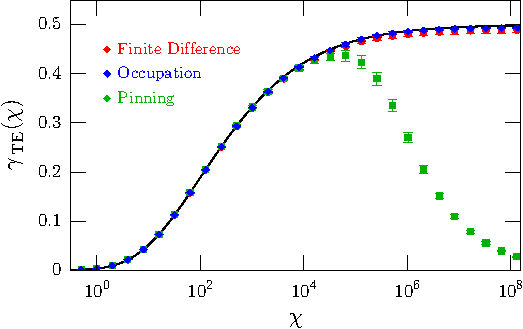
\includegraphics[width=0.8\columnwidth]{fig/numerics/force}
  \caption[Numerically computed TE force]{(Preliminary data) Numerically computed TE force for pinning (squares),
 occupation (circles), and finite difference (squares) methods.
    The finite difference used a step-size $\delta=d/\sqrt{N}$.
    The calculations used $N=10^4$ points per path, and $10^8$ trajectories.}
  \label{fig:force}
\end{figure}
Figure~\ref{fig:force} shows the numerically calculated force on two dielectric planes of equal dielectric
constant, normalized to the total EM force between perfect-conducting plates.
This computation was carried out for the pinning, occupation and finite-difference methods.
In all cases, the paths were generated using the v-loop algorithm~(\ref{eq:unit_vloop}),
and the dielectric path averages were calculated using the trapezoidal method~(\ref{eq:trapezoid}).
Note that in computing path averages for the occupation method, only points \emph{inside} the body
contribute---any points pinned to the surface do not contribute to the dielectric path-average.

The pinning methods discussed in Section~\ref{sec:path-pinning} start to fail for $\chi\gtrsim N$, as expected.
For $\chi\gg N$, the estimate of the force shows the expected $\chi^{-1/2}$ decay.  
For a finite susceptibility, it should be possible to carry out the calculation for large enough $N$, 
but if one is interested in the strong-coupling regime of this theory, then the pinning method is unsuitable.

By contrast, the occupation method is better behaved in the strong-coupling limit.
The occupation-method estimate for the force is computed by generating an initial path $\{\vect{y}_k\}$, 
and translating it via
$\vect{x}_k=\vect{y}_k-\vect{y}_j+\vect{d}$, so that that each point $\vect{x}_j$ lies
on the surface.  The results are then averaged over all such pinnings. 
However, naively implementing this method leads to $N$ evaluations of the path integral, which could
be inefficient.
It may be possible to capture both strong-coupling and general-coupling regimes with only two samples.
First, in order to capture the strong-coupling limit the path integral can be computed for a path where only one point is on the first surface,
and no points are inside the first body.
Second, to capture the remaining $\chi$-dependence, the integrand should be calculated again for a path where a 
randomly selected point is pinned to the first surface, without any constraints on the other occupation numbers.
The strong coupling estimate for the force $f_s$, and the 
general-$\chi$ estimate $f_g$, are combined with weights $N^{-1}$ and $(N-1)/N$ respectively, which
account for enforcing the restrictions.

In the absence of that step to explicitly capture the strong-coupling limit, 
only very rare paths will contribute, since most random paths
starting on the surface are equally like to explore both positive and negative regions. 
Most paths will intersect both bodies, and contribute zero to the force.  For small ensembles ($N_{\text{trial}}\le 10^7$)
this causes similar convergence problems to the pinning methods at large $\chi$. 
However, this would be a statistical error due to insufficient sampling, as opposed to the 
intrinsic problems in the pinning method.  Similar methods will be discussed in more detail
regarding the potential curvature.  

In fact, the general-$\chi$ samples were gathered using stratified sampling, where the path index $k$ was broken into
uniform strata.  This basically splits the sum into multiple pieces and samples from each of those sub-pieces.  For example,
\begin{equation}
  \sum_{k=1}^N a_k = \sum_{j=1}^{N_{\text{strata}}}\sum_{n=1}^{N_{\text{sub}}} a_{n+j\,N_{\text{sub}}},  
\end{equation}
where $N_{\text{sub}}N_{\text{strata}}=N$.
Each stratum was then sampled from uniformly.
In the calculations in Figure~\ref{fig:force}, ten strata were used.  
% The occupation method also has an advantage in that there are no explicit tuning parameters, unlike the finite
% difference.   

Given the deficiencies of the pinning method for finite paths, we will compute the potential
curvature using the occupation method.  
Since the potential curvature requires paths pinned on two different surfaces, 
and will exhibit similar convergence issues at strong coupling, we will develop two different approaches
to generating paths and sampling times.  

\subsection{Direct Path Construction for General-$\chi$ Coupling Method for Potential Curvature}
\label{sec:generic_coupling}

In a method suitable for general coupling, all of the paths start on the surface of the first body,
and are explicitly constructed to intersect the second body after $k$ steps, where the index $k$ is also sampled randomly.  
The paths can be explicitly constructed as Brownian bridges from $x=0$ to $x_k=d$, using Eq.~(\ref{eq:open_vloop}).
The Gaussian factor $\mathcal{G}\big[d,k(N-k)\cT/N^2\big]$ in Eq.~(\ref{eq:curvature_occupy}) is used
to sample path times by treating it and $\cT^{-(1+D/2)}$ as the gamma distribution in $\cT$.  Path times can be sampled 
from Eq.~(\ref{eq:expT}), with $\cT_0=N^2d^2/[2k(N-k)]$ and $a=1+(D+1)/2$.
% The fixed index $k$ for the pinning is determined by randomly selecting from the resulting
% normalization constant.  
% This can be done efficiently by introducing $u:=\cT_0/\cT$, and noting that $u$ is Gamma distributed,
% \begin{equation}
%   P(u;a) = \frac{u^{a-2}}{\Gamma[a-1]}e^{-u}.
% \end{equation}
The pinned point $k$ can be sampled from the combination of $\cT_0^{1-a}$ for normalization $P(\cT)$
and the normalization constant from $\mathcal{G}[d,k(N-k)\cT/N^2]$,  with distribution
\begin{equation}
  P_{\text{pin}}(k;N)=\cN_{\text{pin}} \bigg(\frac{k(N-k)}{N^2}\bigg)^{D/2},
\end{equation}
where $\cN_{\text{pin}} = \sum_{k=1}^NP(k;N)\approx 1/30$ for large $N$.  
In addition for planar surfaces, the integral over the transverse dimensions amounts to an area factor. 

The expression for the potential curvature for general-$\chi$  coupling is
\begin{align}
  C_{ij}=& \frac{\hbar c N }{2(2\pi)^{D/2}}\sum_{k=1}^{N-1}\oint\limits_{\sigma_1(\vect{x}_0-\vect{R}_1)=0} \hspace{-4ex} dS_0\,\biggdlangle 
\oint\limits_{\sigma_2(\vect{x}_k-\vect{R}_2)=0} \hspace{-4ex} dS_k\,\frac{3c'_{N}[\hat{r}_i\cdot\hat{n}_1(\vect{x}_0)][\hat{r}_j\cdot\hat{n}_2(\vect{x}_{k})]}{|\vect{x}_0-\vect{x}_{k}|^{5}}
  \nonumber\\
  &\hspace{2cm} \sum_{n=0}^{N-2}\sum_{m=0}^{N-n-2}\I[1]n\I[2]m g_{m,n}
  \biggdrangle_{k,\cT,\vect{x}_0\leftrightarrow\vect{x}_k},\label{eq:generic_coupling}
\end{align}
where the ensemble average is over path times, pinning separations $k$, and 
Brownian bridges from $\vect{x}_0$ to $\vect{x}_k$, where $\vect{x}_0$ is on the first 
surface, and $\vect{x}_k$ is on the second surface.
% The path times are sampled from $P_{\text{exp-T}}[\cT;\cT_0,1+(D+1)/2]$, with $\cT_0$ given by 
% \begin{equation}
%   \cT_0 = \frac{N^2d^2}{2\Delta(N-\Delta)} \label{eq:T0_curvature}.
% \end{equation}
% The paths are still then constructed subject to the constraints of touching the bodies at the appropriate
% indices.  The remaining integrand is evaluated for the resulting paths.  

In Figure~\ref{fig:curvature_a}, we have used this general-$\chi$ coupling method to compute the potential curvature
without special treatment for strong coupling, with two different ensemble sizes to show the effect of additional averaging.  
%Figure~\ref{fig:curvature_a} shows improved convergence at large $\chi$ once the sample size is increased.  
The general-$\chi$ coupling integrand does eventually lead to the correct answer in the strong-coupling limit once enough
averaging has taken place.  However, achieving that convergence requires a large ensemble to capture the relatively rare, but important,
 paths that just graze both surfaces.
Performance can be improved by introducing separate estimates adapted for the strong-coupling limit.  

This suggests a two-fold approach: First, paths should be generated under the constraint that they touch both surfaces
 without regard for their occupation time (which will capture general $\chi$).  Second, another
set of paths should be generated which just touch the bodies (which will capture large $\chi$).  

\begin{figure}
  \centering
  \includegraphics[width=0.8\columnwidth]{fig/numerics/curvature_a}
  \caption[Numerical TE Potential Curvature for two planar surfaces, evaluated with occupation method]{
    Numerically computed second derivative of potential for two planar surfaces as function 
    of dielectric, for $N=10^5$, each with $10^7$ and $10^9$ trajectories.  
    % While the integrand produces the correct result, recovering the correct answer relies on having a large enough ensemble of 
    % paths, since the strong-coupling limit comes from rare paths.  
    All results are computed using the ``occupation'' method with general-$\chi$ coupling method presented in Eq.~\ref{eq:curvature_occupy}.}
\label{fig:curvature_a}
\end{figure}

\subsection{``Softened'' Delta Function Pinning for Strong-Coupling Limit for Potential Curvature}
\label{sec:softened_delta}
An alternative method to the one presented in Section~(\ref{sec:generic_coupling}),  one more suited to the strong-coupling limit, 
arises from a different treatment of the second delta function $\delta[\sigma_2(\vect{x}_k-\vect{R}_2)]$.
In this case, the first delta function $\delta[\sigma_1(\vect{x}_0-\vect{R}_1 )]$, is still used to pin the paths to start 
on the first body.  Although the paths are assumed to start on the surface of the first body, they do not
enter the bulk of that body.  In order to contribute to the curvature path integral in the strong-coupling limit,
the paths should move towards the second body, and just graze its surface.  

The goal of this method is to develop a way of handling delta function constraints within a path integral
without having to drastically change the way the paths are generated.  This would be particularly
useful for handling pinning in an application involving paths that are hard to construct, such as the TM-Gaussian
paths discussed in Section~\ref{sec:TM-Gaussian}.
In the resulting method, any path can in principle contribute, even if only a few of them 
will give an important contribution.  

\subsubsection{Softened Delta Function Pinning}

Let us consider the term involving $\delta[\sigma_2(\vect{x}_k-\vect{R}_2)]$ from the curvature path integral~(\ref{eq:curvature_occupy}).
After suppressing the integrals over $S_0$ and $\cT$, as well as the leading constants, the remaining spatial path integral
can be written in a schematic form as 
% As an example of the manipulation we propose to use in the curvature path integral~(\ref{eq:curvature_occupy}),
% let us consider the following constrained path integral:
\begin{align}
  I&=\frac{1}{(2\pi\cT)^{D/2}}\biggdlangle \delta[f(\vect{x}_k)]\Phi(\vect{x}_1,\ldots,\vect{x}_{N-1})\biggdrangle_{\vect{x}(t)}\\
  &= \int \prod_{n=1}^{N-1}d\vect{x}_n\, \prod_{k=0}^{N-1}\bigg(\frac{e^{-(\vect{x}_{k+1}-\vect{x}_k)^2/(2\Delta \cT)}}{
    (2\pi\Delta \cT)^{D/2}}\bigg)\delta[f(\vect{x}_k)]\Phi(\vect{x}_1,\ldots,\vect{x}_{N-1}),\label{eq:constrain_int}
\end{align}
where $f(\vect{x}_k)$ and $\Phi$ are placeholders for the constraint $\sigma_2(\vect{x}_k-\vect{R}_2)$, 
integrand $\sum_n\sum_m\I[1]m\I[2]n g_{m,n}$, respectively.  There is no Gaussian term,
 since that only arises after pinning the paths, and normalizing
for pinned Brownian bridges.   

Instead of just evaluating the integral over $\vect{x}_k$ (which pins the paths), the integral can
be multiplied by a factor of unity of the form:
\begin{equation}
  1 = \dfrac{(2\pi\Delta \cT)^{-D}\int d\vect{y}_k\, e^{-(\vect{x}_{k+1}-\vect{y}_k)^2/(2\Delta \cT)-(\vect{y}_{k}-\vect{x}_{k-1})^2/(2\Delta \cT)}}{
    (4\pi\Delta T)^{-D/2}\,e^{-(\vect{x}_{k+1}-\vect{x}_{k-1})^2/(4\Delta \cT)}}.\label{eq:fac_one}
\end{equation}
This involves multiplying and dividing by an unconstrained integral connecting $\vect{x}_{k-1}$
and $\vect{x}_{k+1}$ via a new coordinate $\vect{y}_k$.  The integral has been evaluated in the denominator.  
Then the constrained integral~(\ref{eq:constrain_int}) can now be written
\begin{align}
  I&= \int d\vect{y}_k\int \prod_{n=1}^{N-1}d\vect{x}_n\, \prod_{k=0}^{N-1}\bigg(\frac{e^{-(\vect{x}_{k+1}-\vect{x}_k)^2/(2\Delta \cT)}}
  {(2\pi\Delta \cT)^{D/2}}\bigg) \frac{e^{-(\vect{x}_{k+1}-\vect{y}_k)^2/(2\Delta \cT)-(\vect{y}_{k}-\vect{x}_{k-1})^2/(2\Delta \cT)}}{(2\pi\Delta\cT)^{D}}\nonumber\\
  &\hspace{0.5cm}\times    (4\pi\Delta T)^{D/2}\,e^{(\vect{x}_{k+1}-\vect{x}_{k-1})^2/(4\Delta \cT)}
  \delta[f(\vect{x}_k)]\Phi(\vect{x}_1,\ldots,\vect{x}_k,\ldots,\vect{x}_{N-1}).
\end{align}
The label for the constrained coordinate $\vect{x}_k$ and the unconstrained coordinate $\vect{y}_k$ can be swapped using $\vect{x}_k\leftrightarrow\vect{y}_k$.
The unconstrained coordinates $\vect{x}_k$ will then be used with all of the other coordinates to create free Brownian bridges,
and $\delta[f(\vect{y}_k)]$ is now isolated in an auxiliary integral.  
%The Gaussian factors in $\vect{y}_k-\vect{x}_{k+1}$ can be swapped with their counterparts involving $\vect{x}_k-\vect{x}_{k+1}$.
The path integral can be written in ensemble-averaged form,
\begin{align}
  I&= \frac{1}{(2\pi\cT)^{D/2}}\biggdlangle \int d\vect{y}_k \frac{e^{-(\vect{y}_{k}-\bar{\vect{x}}_k)^2/\Delta \cT}}
  {(\pi\Delta \cT)^{D/2}}\delta[f(\vect{y}_k)]\Phi(\vect{x}_1,\ldots,\vect{y}_k,\ldots,\vect{x}_{N-1})\biggdrangle,
\end{align}
where $\vect{\bar{x}}_k:=(\vect{x}_{k-1}+\vect{x}_{k+1})^2$, and the exponential terms were combined using
\begin{align}
&  (\vect{x}_{k+1}-\vect{y}_k)^2+(\vect{y}_{k}-\vect{x}_{k-1})^2 -\frac{(\vect{x}_{k+1}-\vect{x}_{k-1})^2}{2}%\nonumber\\
% &=  \vect{x}_{k+1}^2-2\vect{x}_{k+1}\cdot\vect{y}_k+\vect{y}_k^2
% +\vect{x}_{k-1}^2-2\vect{x}_{k-1}\cdot\vect{y}_k+\vect{y}_k^2
%  -\frac{(\vect{x}^2_{k+1}-2\vect{x}_{k+1}\cdot\vect{x}_{k-1}+\vect{x}_{k-1}^2}{2}\nonumber\\
% &=  \frac{(\vect{x}_{k+1}+\vect{x}_{k-1})^2}{2}-2\vect{x}_{k+1}\cdot\vect{y}_k+2\vect{y}_k^2
% -2\vect{x}_{k-1}\cdot\vect{y}_k
%  \nonumber\\
% &=  \frac{(\vect{x}_{k+1}+\vect{x}_{k-1})^2}{2}-2(\vect{x}_{k+1}+\vect{x}_{k-1})\cdot\vect{y}_k+2\vect{y}_k^2
% -2\vect{x}_{k-1}\cdot\vect{y}_k\\
=  2(\vect{y}-\vect{\bar{x}}_k)^2.
\end{align}
Now the delta function can be integrated over using Eq.~(\ref{hormander1}), with the result 
\begin{align}
  I&= \frac{1}{(2\pi\cT)^{D/2}}\biggdlangle \oint_{f(\vect{y})=0} \hspace{-4ex}dS(\vect{y})\, \frac{1}{|\nabla_yf(\vect{y})|}\frac{e^{-(\vect{y}-\bar{\vect{x}}_k)^2/\Delta \cT}}
  {(\pi\Delta \cT)^{D/2}}\Phi(\vect{x}_1,\ldots,\vect{y},\ldots,\vect{x}_{N-1})\biggdrangle_{\vect{x}(t)}.\label{eq:soft_delta_general}
\end{align}
There is an integral over the surface of constraint $f(\vect{y})$, and the functional $\Phi$ is constrained such that 
its $k$th coordinate is on the surface.  The paths can be  constructed without any concern for the constraints,
but they will be suppressed by the Gaussian if they strongly violate the constraint that $\vect{y}\sim\vect{\bar{x}}_k$.  
In effect, this manipulation has ``softened'' the constraints. Previously, $\vect{x}_k$ had to lie exactly on the 
surface, whereas now $\bar{\vect{x}}_k$ should be within $\sqrt{\Delta \cT}$ of the surface to contribute to the path
integral.  
Since a broader class of paths can be considered, it maybe easier to find sample paths where 
that almost obey the constraint $\vect{y}\sim\vect{\bar{x}}_k$.
Those paths can then contribute to the path integral in regions where $\Phi$ is nonzero.     

\subsubsection{Splitting the Potential Curvature}

Since the strong-coupling limit in the curvature~(\ref{eq:curvature_occupy}) 
comes from the terms proportional to $\I[1]0\I[2]0$, 
those terms can be separated out, and treated using the softened delta function approach.
The remaining terms will be treated using the generic coupling discussed in Section~\ref{sec:generic_coupling}.
The curvature can be split into a strong-coupling and general-$\chi$ coupling term
\begin{align}
  C_{ij} =\,& C_{ij}^{(\text{S})} + C_{ij}^{(\text{g})},
\end{align}
where the strong-coupling term is
\begin{align}
C^{(\text{S})}_{ij}&=\frac{\hbar c N}{2(2\pi)^{D/2}}\intzinf\frac{d\cT}{\cT^{1+D/2}}
 \oint\limits_{\sigma_1(\vect{x}_0-\vect{R}_1)=0}  \hspace{-4ex} dS_0\, 
  \hat{r}_i\cdot\hat{n}_1(\vect{x}_0)
 \oint\limits_{\sigma_2(\vect{y}-\vect{R}_2)=0}  \hspace{-4ex} dS(\vect{y})\, 
  \hat{r}_j\cdot\hat{n}_2(\vect{y})
  \nonumber\\
&\hspace{0.5cm}\times\biggdlangle 
\sum_{k=1}^{N-1}\frac{e^{-(\vect{y}-\bar{\vect{x}}_k)^2/\Delta \cT}}  {(\pi\Delta \cT)^{D/2}}
  \I[1]0\,\I[2]0\, g_{0,0}
  \biggdrangle_{\vect{x}(t)},\label{eq:curvature_strong}
\end{align}
and the general-$\chi$ coupling term $C^{(\text{g})}_{ij}$ is
\begin{align}
C^{\text{(g)}}_{ij}
=& \frac{\hbar c N}{2(2\pi)^{D/2}}\sum_{k=1}^{N-1}\intzinf\frac{d\cT}{\cT^{1+D/2}}
  % \nonumber\\ 
  % &\times
 \oint\limits_{\sigma_1(\vect{x}_0-\vect{R}_1)=0}  \hspace{-4ex} dS_0\, 
  \hat{r}_i\cdot\hat{n}_1(\vect{x}_0)
 \oint\limits_{\sigma_2(\vect{x}_k-\vect{R}_2)=0}  \hspace{-4ex} dS_k\, 
  \hat{r}_j\cdot\hat{n}_2(\vect{x}_k)
  \nonumber\\
&\times\sum_{m,n\ne 0}\biggdlangle 
  \mathcal{G}(\vect{x}_0-\vect{x}_k,k(N-k)\cT/N^2)
  % \nonumber\\
  % &\hspace{0.75cm} \times
  \I[1]m\,\I[2]n\, g_{m,n}
  \biggdrangle_{\sigma_2(\vect{x}_k-\vect{R}_2)=0},\label{eq:curvature_generic}
\end{align}
The integral~(\ref{eq:curvature_strong}) is only substantially nonzero under two conditions.
First, the path must pass within a distance $\sqrt{\Delta\cT}$ of the 
surface, and second the paths must not enter either body.
Note that due to the pinning, the indicator functions $\I[1]0\,\I[2]0$ are currently defined with $\vect{y}$ in the $k$th spot.
This means that if $\vect{x}_k$ lies inside either body, that does not influence the integrand.  
The indicators only go to zero when one of the \emph{other} points on the path cross into the bodies.  

In a planar geometry, the $(D-2)$-dimensional surface integrals can be evaluated.  
The integral over $S(\vect{y})$ eliminates the transverse Gaussian integrals, and 
integral over the starting surface gives a factor of the transverse area.  
In $D=4$ dimensions, Eq.~(\ref{eq:curvature_strong}) then simplifies to 
\begin{align}
C^{(\text{S})}_{ij}&=\frac{\hbar c N A}{2(2\pi)^{2}}\intzinf\frac{d\cT}{\cT^{3}}\biggdlangle 
  \sum_{k=1}^{N-1}\frac{e^{-(d_2-\bar{x}_k)^2/\Delta \cT}}  {(\pi\Delta \cT)^{1/2}}
  \I[1]0\,\I[2]0\, g_{0,0}
  \biggdrangle_{x(t),x_0=d_1},\label{eq:curvature_strong_simple}
\end{align}
In order to capture the strong-coupling dependence it is necessary to sample from the 
set of paths that do not enter either body.  For two dielectric planes with dielectric function~(\ref{eq:eps12})
the paths can be constructed by shifting the paths so they start on the 
first surface at $x=d_1$.   
For paths constructed by scaling unit Brownian bridges, $x_k=d_1+\sqrt{\cT}B_k$,
this can be done by translating the unit Brownian bridge $B(t)\rightarrow B(t) -B_{\text{min}}$,
where $B_{\text{min}}$ is the minimum value of the path.  This ensures that 
the paths start at $x=d_1$, but since $\sqrt{\cT}B(t)>0$ for all points of the path, the paths 
will not enter the first body.    
Then suppose that the maximum point of the bridge is $B_{\text{max}}$, and the maximum point of the 
path is $x_{\text{max}}=d_1+\sqrt{\cT}B_{\text{max}}$.  Only this point will have 
an opportunity to contribute.  Once it passes through the surface, $\I[1]0\I[2]0$ is zero, and 
so the integrand is also zero.  
Then the Gaussian $e^{-(d_2-\bar{x}_{\text{max}})^2/\Delta \cT}$ can be used to sample a path-time, 
while ensuring that the path does not actually enter the surface.  
That crossing time $\cT_{\text{max}}$ definitely happens when $\sqrt{\cT_{\text{max}}}B_{\text{max}}=d$, where $d=d_2-d_1$.  
The exponential factor in Eq.~(\ref{eq:curvature_strong_simple}) can be written using the definition of $x_{\text{max}}$ 
as
\begin{align}
  \exp\bigg(-\frac{1}{\Delta \cT}[d-\sqrt{\cT}\bar{B}_{\text{max}}]^2\bigg) 
  &= \exp\bigg[-Nd^2\bigg(\frac{1}{\sqrt{\cT}}-\frac{\bar{B}_\text{max}}{d}\bigg)^2\bigg],
\end{align}
where $\bar{B}_\text{max} := (B_{m^*+1}-B_{m^*-1})/2$, and $m^*$ is the index of the maximum value.
This can be regarded as the probability distribution for $\cT$.  
The normalized probability distribution for $1/\sqrt{\cT}$ is  
\begin{equation}
  P_S(\cT;\bar{B}_\text{max},d,N) = \sqrt{\frac{Nd^2}{\pi\cT^3}}\exp\bigg[-Nd^2\left(\frac{1}{\sqrt{\cT}}-\frac{\bar{B}_\text{max}}{d}\right)^2\bigg]\Theta\left(\frac{d^2}{\bar{B}^2_\text{max}}-\cT\right)
  \label{eq:time_fix_curve}
\end{equation}
The probability distribution can simplified by defining
\begin{equation}
  s = \sqrt{2Nd^2}\left(\frac{1}{\sqrt{\cT}}-\frac{\bar{B}_\text{max}}{d}\right),
\end{equation}
where 
\begin{equation}
  P_S(s) = \bigg| \frac{dT}{ds}\bigg| P_S(\cT) = \sqrt{\frac{2}{\pi}} e^{-s^2/2}\Theta(s),
\end{equation}
is a one-sided normal distribution.  In this case, $s$ is the absolute value of a standard normal deviate, and 
the path times can be written in terms of standard normal deviates as
\begin{equation}
  \cT = \left( \frac{|z|}{\sqrt{2Nd^2}}+\frac{\bar{B}_\text{max}}{d}\right)^{-2}\label{eq:cT-s}.
\end{equation}
The $\cT$ integral will be computed in Monte Carlo fashion after factoring out the probability density~(\ref{eq:time_fix_curve}),
and using Eq.~(\ref{eq:cT-s}).  The sum over $k$ is assumed to be dominated by the contribution at the maximum point,  
\begin{align}
C^{(S)}_{ij} % &=\frac{\hbar c N A}{2(2\pi)^{2}}\biggdlangle 
  % \intzinf\frac{d\cT}{\cT^{3}}\sqrt{\frac{\pi\cT^3}{Nd^2}}\sqrt{\frac{N}{\pi \cT}}\bigg(\sqrt{\frac{Nd^2}{\pi\cT^3}}e^{-(d_2-\bar{x}_k)^2/\Delta \cT}\bigg)
  % \I[1]0\,\I[2]0\, g_{0,0}
  % \biggdrangle_{\vect{x}(\cT),x_0=d_1},\\
 &=\frac{\hbar c N A}{2(2\pi)^{2}}\biggdlangle 
 \frac{1}{\cT^{2}d}\bigg(\sqrt{\frac{Nd^2}{\pi\cT^3}}e^{-(d_2-\bar{x}_\text{max})^2/\Delta \cT}\bigg)
  \I[1]0\,\I[2]0\, g_{0,0}
  \biggdrangle_{\vect{x}(\cT),x_0=d_1}.\label{eq:strong_coupling_final}
\end{align}
Note that there is no explicit pinning on the paths, but this integrand is only non-zero 
if the paths do not enter the bodies.  

\begin{figure}
  \centering
  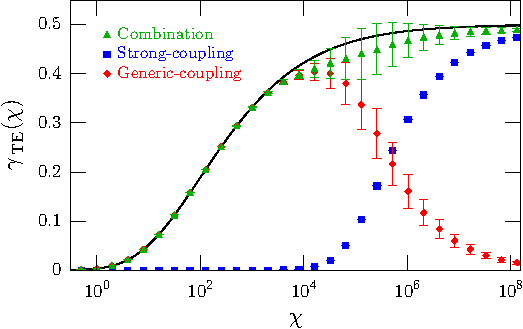
\includegraphics[width=0.8\columnwidth]{fig/numerics/curvature_c}
  \caption[(Preliminary data) Numerical TE Potential Curvature for two planar surfaces, evaluated with strong-coupling methods]{
(Preliminary data) Numerically computed second derivative of TE potential for two planar surfaces as function 
    of dielectric, for $N=10^5$, with $10^8$ trajectories.
    Strong coupling results are shown as blue squares, generic coupling as red diamonds, 
    and their sum as green triangles.  
    All simulations are computed using
  ``occupation'' method in Eq.~\ref{eq:curvature_occupy}, and both estimates use the the same ensemble of random numbers.}
\label{fig:curvature_c}
\end{figure}

Figure~\ref{fig:curvature_c} shows the effects of including the strong coupling term~(\ref{eq:strong_coupling_final}).  
The strong-coupling term only becomes important for $\chi/N\gg 1$,
and there is a transition between the generic coupling and strong-coupling regimes. 
The variance of the total estimated potential is also increased in the cross-over region, 
dominated by the statistical error from the generic coupling estimate.  
The method used here manages to improve on the generic coupling results significantly, since 
it does not rely on rare paths from a very large ensemble to capture the behavior in the strong-coupling regime.
However, the presented results have a larger statistical error than the simpler generic coupling, but this is 
perhaps due to a slightly smaller ensemble of paths.  There are $N=10^8$ sample paths in Figure~\ref{fig:curvature_c}, versus $N=10^9$ 
sample paths in Figure~\ref{fig:curvature_a}.  This is
still under study.   

There is yet another way of treating the delta function in terms of restricting $\cT$. 
If the paths are assumed to start on the surface of the first body, and not enter, 
then the delta function can be interpreted as a delta function in the path time $\cT$. 
(Since there is only one $\cT$ integral in the path integral, only one of the $\delta$ functions can be handled in this manner.
The remainder should be accounted for in the spatial integrals.)
For a given Brownian bridge $\vect{B}_k$, the times $\cT_*$ that it intersects the  surfaces, or 
satisfies $\sigma_2(\vect{x}_0+\sqrt{\cT_*}\vect{B}_k-\vect{R}_2)=0$ could be found.  
This has not yet been fully implemented, but would be much simpler.  However, the softened delta function
approach may be also be useful in handling other constraints.    For example, it may be useful when 
computing the potential in a complicated geometry.  It might be hard to construct paths that 
touch both surfaces, and yet enter neither from randomly constructing Brownian bridges.
This softened style of pinning could allow a broader class of paths to contribute in that case.    


%%% Local Variables: 
%%% mode: latex
%%% TeX-master: "thesis_master"
%%% End: 
